% !TEX TS-program = pdflatex
% ACM Article template (sigconf) – nonacm & review per Vorgabe
\documentclass[sigconf,nonacm,review]{acmart}

% ====== Packages ======
\usepackage[utf8]{inputenc}
\usepackage[T1]{fontenc}
\usepackage[ngerman]{babel}

\usepackage{graphicx}
\graphicspath{{figs/}}
\DeclareGraphicsExtensions{.pdf,.png,.jpg}  
\usepackage{microtype}
\usepackage{xcolor}
\usepackage{enumitem}
\setlist{nosep}
\usepackage{float}
\usepackage{placeins}


\title{Abschlussreport Fachprojekt Routingalgorithmen}
\subtitle{TE\_SR\_WAN\_simulation \& TE\_SR\_experiments}

\author{Marcel Gerhardt}
\affiliation{\institution{TU Dortmund}\city{}\country{}}
\author{Ayoub Lahrach}
\affiliation{\institution{TU Dortmund}\city{}\country{}}
\author{Xiaoyu Zhou}
\affiliation{\institution{TU Dortmund}\city{}\country{}}

\renewcommand\shortauthors{Gerhardt, Lahrach, Zhou}

\thanks{Betreuung / Lehrstuhl: Prof. Dr. Dr. Klaus-Tycho Förster \quad Datum: 22.09.2025}

\settopmatter{printacmref=false}
\pagestyle{plain}

\begin{document}

\begin{abstract}
In diesem Fachprojekt entwickeln und evaluieren wir zwei Ansätze zur Reduktion der maximalen Linkauslastung (MLU) in Weitverkehrsnetzen: (i) \textbf{TL\_Inverse}, eine auslastungsadaptive Erweiterung der klassischen \emph{inverse\_capacity}-Heuristik, und (ii) eine kapazitätsbewusste Demand-First-Waypoints-Variante \textbf{(DFW)} auf Basis von \emph{Demand-First-Waypoints} mit inverse\_capacity-Initialisierung und robustem ECMP-Splitting. In \textit{Projekt~1 (TE\_SR\_WAN\_simulation)} untersuchen wir beide Verfahren auf den Topologien \textbf{Abilene}, \textbf{Géant} und \textbf{Germany50} und vergleichen sie jeweils mit ihren Baselines. Die Ergebnisse zeigen topologieabhängige Vorteile: \textbf{TL\_Inverse} senkt die MLU insbesondere in gut vernetzten Netzen (z.\,B. Géant), während \textbf{DFW} in Szenarien mit hinreichender Pfaddiversität leichte Mediangewinne erzielt, jedoch mit höherer Streuung. In \textit{Projekt~2 (TE\_SR\_experiments)} entwerfen wir eine kompakte, SR-fähige Topologie mit bewusstem Innen-Bottleneck und vergleichen \textbf{TL\_Inverse} gegen eine statisch getunte Dijkstra-Baseline (\textbf{New\_Weights}) sowie \textbf{DFW} gegen eine \textbf{Weights}-Baseline. Beide Experimente werten wir über Boxplots der MLU aus. Abschließend replizieren wir die Resultate einer anderen Gruppe für beide Projektteile erfolgreich. Die verwendeten und erstellten Repositories sind am Ende gelistet.
\end{abstract}

\maketitle


\section{Einleitung \& Ziele}
Traffic Engineering (TE) zielt auf eine Lastverteilung, die Engpässe vermeidet und vorhandene Kapazitäten effizient nutzt. Eine zentrale Zielgröße ist die \emph{maximale Linkauslastung (MLU)}, d.\,h.\ der maximale Quotient aus Last und Kapazität über alle Kanten. Dieser Report adressiert zwei komplementäre algorithmische Ansätze zur MLU-Reduktion: \textbf{(i)} \emph{TL\_Inverse} als auslastungsadaptive Erweiterung von \emph{inverse\_capacity} und \textbf{(ii)} eine kapazitätsbewusste Demand-First-Waypoints-Variante \textbf{(DFW)} mit \emph{inverse\_capacity}-Initialisierung und robustem ECMP-Splitting.

Im Mittelpunkt stehen die Entwicklung und Evaluation von \textbf{TL\_Inverse} und \textbf{DFW} auf den Topologien \textbf{Abilene}, \textbf{Géant} und \textbf{Germany50}, jeweils im Vergleich zu ihren Baselines. Darauf aufbauend übertragen wir beide Ansätze in ein zweites, SR-fähiges Repository mit eigens entworfener Topologie, wobei \textbf{TL\_Inverse} gegen \textbf{New\_Weights} und \textbf{DFW} gegen eine \textbf{Weights}-Baseline antritt. Abschließend prüfen wir die Reproduzierbarkeit, indem wir Resultate einer anderen Projektgruppe nachvollziehen und einordnen.



\section{Hintergrund}

\textbf{Dijkstra / ECMP:}
Kürzeste-Wege-Routing minimiert die Summe der Kantengewichte entlang eines Pfads.
Existieren mehrere Pfade mit identischer Gesamtkostenlänge, aktiviert \emph{Equal-Cost Multi-Path} (ECMP)
eine gleichmäßige Aufteilung des Demand-Volumens auf diese Pfade. Formal: Für Gewichte $w$ und Demand $(s,t,d)$
bezeichne $a_{ij}(s,t;w)\in[0,1]$ den ECMP-Anteil auf Link $(i,j)$; die linkweise Last ist
$\ell_{ij}(w)=\sum_{(s,t,d)\in\mathcal D} d\,a_{ij}(s,t;w)$.

\textbf{inverse\_capacity (IC):}
Linkkosten werden proportional zum Kehrwert der Kapazität gesetzt, skaliert über die maximale Kapazität:
\[
\mathrm{base\_w}_{ij}=\frac{\max_{e\in E}c_e}{c_{ij}}\!,
\]
wodurch kapazitätsstarke Links in der Kürzeste-Wege-Metrik bevorzugt werden. IC dient bei uns sowohl als Baseline
(ohne weitere Anpassung) als auch als Startmetrik für adaptive Verfahren.

\textbf{TL\_Inverse:}
Aufbauend auf IC werden die Gewichte \emph{iterativ} relativ zur Basis an die beobachtete, normierte Auslastung
$u_{ij}=\ell_{ij}/c_{ij}$ angepasst:
\[
w^{(k+1)}_{ij}=\mathrm{base\_w}_{ij}\,\bigl(1+\alpha\,u^{(k)}_{ij}\bigr),\quad \alpha>0.
\]
Ablauf: Routen $\rightarrow$ Last messen $\rightarrow$ Gewichte anpassen (mehrere Iterationen, dann Fixierung).
Die Skalierung \emph{relativ zur Basis} begrenzt Übersteuerung und stabilisiert das Verfahren.

\textbf{Demand-First-Waypoints Prinzip:}
Greedy-Heuristik mit \emph{höchstens einem} Waypoint (Segment) pro Demand: Demands werden \emph{absteigend nach Volumen}
bearbeitet; für jeden Demand $(s,t,d)$ wird ein Kandidat $w\in V\setminus\{s,t\}$ gesucht, der die
\emph{maximale Linkauslastung (MLU)} 
\[
\mathrm{MLU}(w)=\max_{(i,j)\in E}\frac{\ell_{ij}(w)}{c_{ij}}
\]
möglichst senkt (Routing über $s\!\to\!w\!\to\!t$ mit Dijkstra+ECMP). Nur wenn die MLU \emph{strikt} sinkt, wird $w$ akzeptiert;
anschließend wird die Lastkarte aktualisiert.

\textbf{DFW-Variante (DFW):}
Zwei gezielte Modifikationen:
(i) \emph{Kapazitätsbewusste Startmetrik} via IC (siehe oben) statt uniformer Kosten, damit die Waypoint-Suche auf Pfade mit
mehr „Headroom“ fokussiert.
(ii) \emph{Robuster ECMP-Split}: Sonderfall „keine gültigen Nachfolger“ führt nicht zu Division durch Null; Pfadanteile werden
deterministisch auf 0 gesetzt. Greedy-Schema, MLU-Kriterium und ECMP bleiben unverändert.

\textbf{Topologien.}
\emph{Abilene} (klein, relativ homogen; geringe Pfaddiversität), \emph{Géant} (mittelgroß, gut vernetzt; mehrere
konkurrenzfähige Alternativrouten), \emph{Germany50} (größer, heterogener; höhere Sensitivität für Parameter und Heuristiken).


\section{Projekt 1\,\textemdash\,TE\_SR\_WAN\_simulation}
\subsection{Algorithmus \texorpdfstring{\textbf{TL\_Inverse}}{TL_Inverse}}
Wir modellieren das Netzwerk als gerichteten Graphen $G=(V,E)$ mit Linkkapazitäten $c_{ij}>0$ für $(i,j)\in E$ und einer Demandmenge
$\mathcal{D}=\{(s,t,d)\}$, wobei $d$ das zu routende Verkehrsvolumen von Quelle $s$ zu Senke $t$ bezeichnet. Ausgehend von der klassischen
\emph{inverse\_capacity}-Heuristik werden zunächst \emph{Basisgewichte} definiert, die Links mit hoher Kapazität begünstigen:
\begin{equation}
\mathrm{base\_w}_{ij} \;=\; \frac{\max_{e\in E} c_e}{c_{ij}}
\quad\text{für alle }(i,j)\in E.
\label{eq:basew}
\end{equation}
Diese Basiskosten dienen als Ausgangspunkt eines iterativen, lastsensitiven Anpassungsverfahrens. Wir initialisieren $w^{(0)}_{ij}=\mathrm{base\_w}_{ij}$ und berechnen
für jede Iteration $k=0,\dots,K-1$ zunächst die kürzesten Wege relativ zu den aktuellen Gewichten $w^{(k)}$. Bei Mehrdeutigkeit (gleich lange Pfade)
verwenden wir ECMP und teilen das Volumen $d$ eines Demands gleichmäßig auf alle gleichwertigen Pfade auf. Bezeichne $a^{(k)}_{ij}(s,t)\in[0,1]$
den Anteil des Demands $(s,t,d)$, der in Iteration $k$ über Link $(i,j)$ fließt (ECMP-Anteilssplitting). Daraus ergibt sich die linkweise
\emph{akkumulierte Last}
\begin{equation}
\ell^{(k)}_{ij} \;=\; \sum_{(s,t,d)\in\mathcal{D}} d \cdot a^{(k)}_{ij}(s,t),
\label{eq:load}
\end{equation}
und die \emph{normierte Auslastung}
\begin{equation}
u^{(k)}_{ij} \;=\; \frac{\ell^{(k)}_{ij}}{c_{ij}}\,.
\label{eq:util}
\end{equation}
Im Anschluss werden die Linkgewichte proportional zur beobachteten Auslastung angepasst. Charakteristisch für \textit{TL\_Inverse} ist dabei,
dass die Aktualisierung stets \emph{relativ zur Basisgewichtung} (\ref{eq:basew}) erfolgt und somit keine ungebundene Gewichtsausweitung
über Iterationen hinweg stattfinden kann:
\begin{equation}
w^{(k+1)}_{ij} \;=\; \mathrm{base\_w}_{ij}\,\bigl(1 + \alpha\,u^{(k)}_{ij}\bigr),
\quad\alpha>0.
\label{eq:update}
\end{equation}
Der Parameter $\alpha$ steuert die Reaktionsstärke des Verfahrens: Kleine Werte führen zu konservativen, große Werte zu aggressiveren
Gewichtsanhebungen auf ausgelasteten Links. Nach $K$ Iterationen (in unseren Experimenten typischerweise $K=3$) werden die finalen Gewichte
$w^{\star}_{ij}=w^{(K)}_{ij}$ fixiert, und die endgültige Routenwahl erfolgt wieder per ECMP über kürzeste Pfade. Durch die Skalierung relativ
zur Basis (\ref{eq:basew}) bleibt das Verfahren numerisch stabil, während (\ref{eq:update}) gezielt jene Links penalisiert, deren
normierte Auslastung (\ref{eq:util}) in der vorherigen Iteration erhöht war. Auf diese Weise können Hotspots schrittweise entschärft und
Verkehrslasten auf weniger beanspruchte Teile der Topologie umverteilt werden.

\subsection{Evaluationsdesign (TL\_Inverse)}
Zur Beurteilung von \textit{TL\_Inverse} vergleichen wir das Verfahren gegen die klassische
\emph{inverse\_capacity}\,-Baseline auf drei etablierten WAN-Topologien:
\textbf{Abilene} (klein, relativ homogen), \textbf{Géant} (mittelgroß, gut vernetzt) und
\textbf{Germany50} (größer, heterogener). Als Verkehrsgrundlage dienen realistisch skalierte
Demand-Matrizen; geroutet wird stets auf einem gerichteten Graphen $G=(V,E)$ mit Kapazitäten
$c_{ij}>0$ für $(i,j)\in E$. Für \textit{TL\_Inverse} werden die Gewichte aus der in
Abschnitt~3.1 beschriebenen Iterationsprozedur gewonnen (typisch $K=3$ Iterationen) und für
die finale Bewertung fixiert. Die Baseline \emph{inverse\_capacity} entsteht aus den
Basisgewichten $\mathrm{base\_w}_{ij}=\max_{e\in E}c_e/c_{ij}$ ohne weitere Anpassung.

Die Routenwahl erfolgt deterministisch mittels kürzester Wege relativ zu den finalen Gewichten
und \emph{Equal-Cost Multi-Path} (ECMP): Existieren mehrere gleichlange Pfade, wird das
Demand-Volumen $d$ eines Paares $(s,t,d)$ gleichmäßig auf diese Pfade verteilt. Bezeichne
$a_{ij}(s,t;w)\in[0,1]$ den ECMP-Anteil des Demands $(s,t,d)$, der unter Gewichten $w$ über
Link $(i,j)$ fließt. Dann ergibt sich die linkweise Last zu
\[
\ell_{ij}(w)\;=\;\sum_{(s,t,d)\in\mathcal D} d\cdot a_{ij}(s,t;w)\,,
\]
die \emph{normierte Auslastung} zu $u_{ij}(w)=\ell_{ij}(w)/c_{ij}$ und als zentrale Zielgröße
die \emph{maximale Linkauslastung} (MLU)
\[
\mathrm{MLU}(w)\;=\;\max_{(i,j)\in E}\,u_{ij}(w)\,.
\]
Für \textit{TL\_Inverse} variieren wir die Reaktionsstärke über
$\alpha\in\{0.3,\,0.5,\,0.7\}$; die übrigen Parameter (Topologie, Kapazitäten, Demands,
Routingmodell) bleiben zwischen den Algorithmen identisch. Ergebnisse berichten wir als
Abbildungen (Balken/Boxplots) je Topologie und $\alpha$; auf Tabellen verzichten wir bewusst,
da der Fokus auf der qualitativen Einordnung der MLU-Unterschiede liegt. Hinweise auf weitere
Heuristiken (z.\,B. \emph{DemandFirstWaypoints/GreedyWaypoints}) erscheinen in einzelnen
Abbildungen nur als Kontext und sind nicht Teil der primären Bewertung.

\subsection{Ergebnisse (TL\_Inverse)}
\begin{figure}[H]
  \centering
  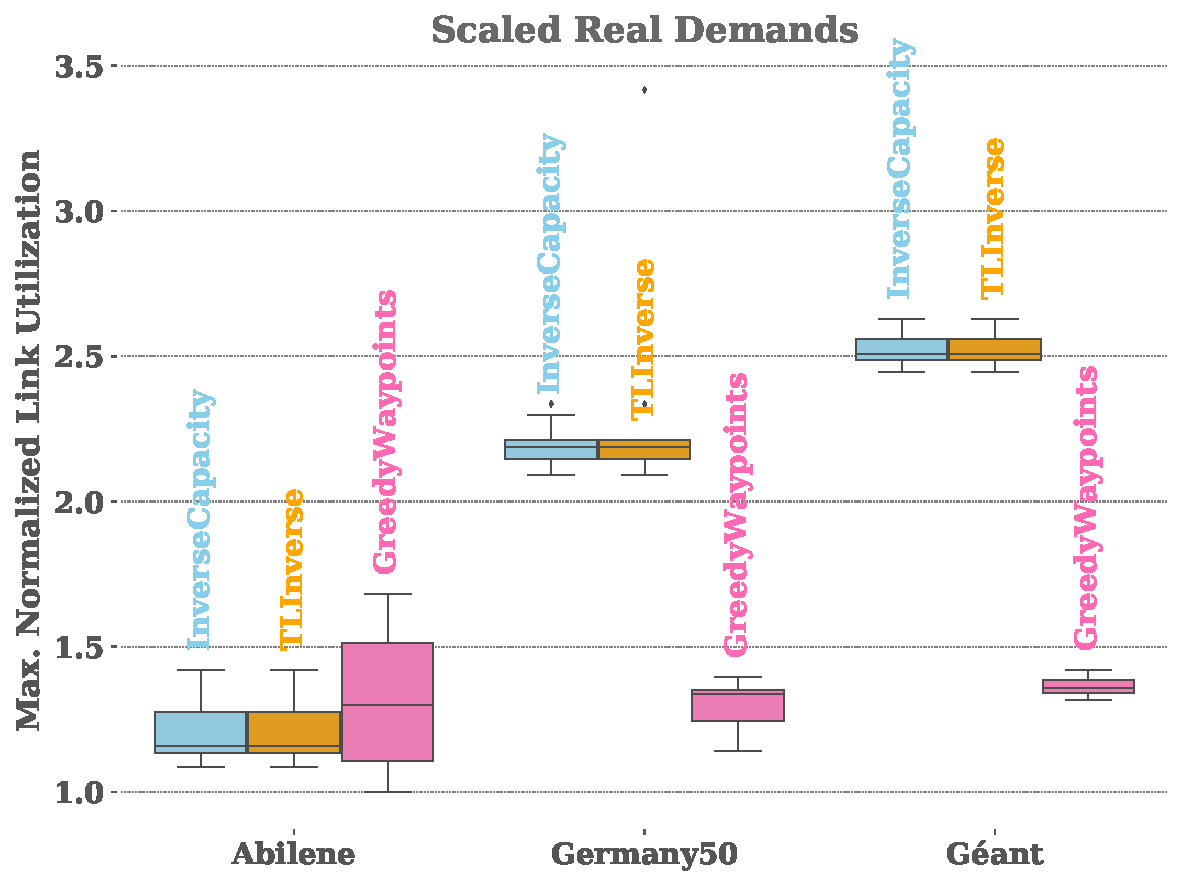
\includegraphics[width=.95\linewidth]{p1_alpha_03.pdf}
  \caption{Projekt 1 -  TL\_Inverse, $\alpha=0{,}3$}
  \label{fig:p1-a03}
\end{figure}
\begin{figure}[H]
  \centering
  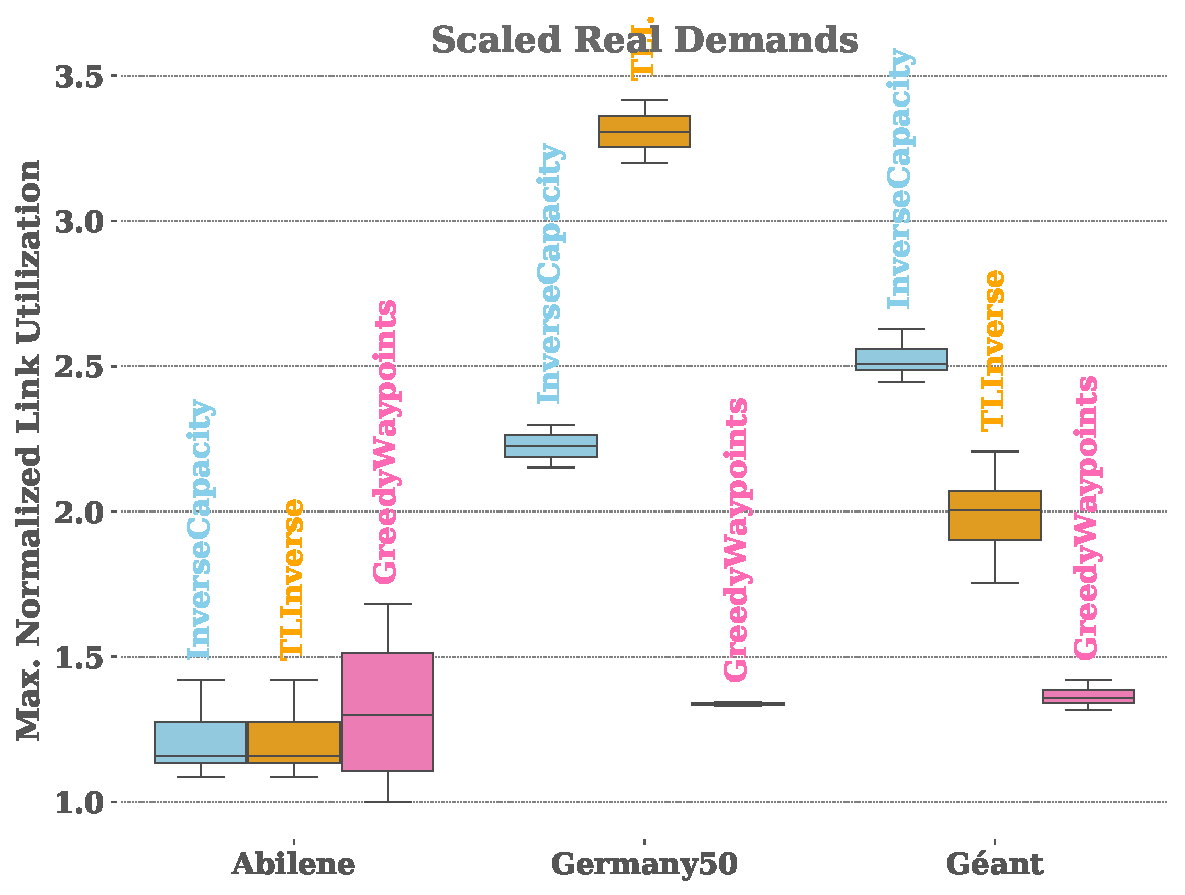
\includegraphics[width=.95\linewidth]{p1_alpha_05.pdf}
  \caption{Projekt 1 – TL\_Inverse, $\alpha=0{,}5$}
  \label{fig:p1-a05}
\end{figure}
\begin{figure}[H]
  \centering
  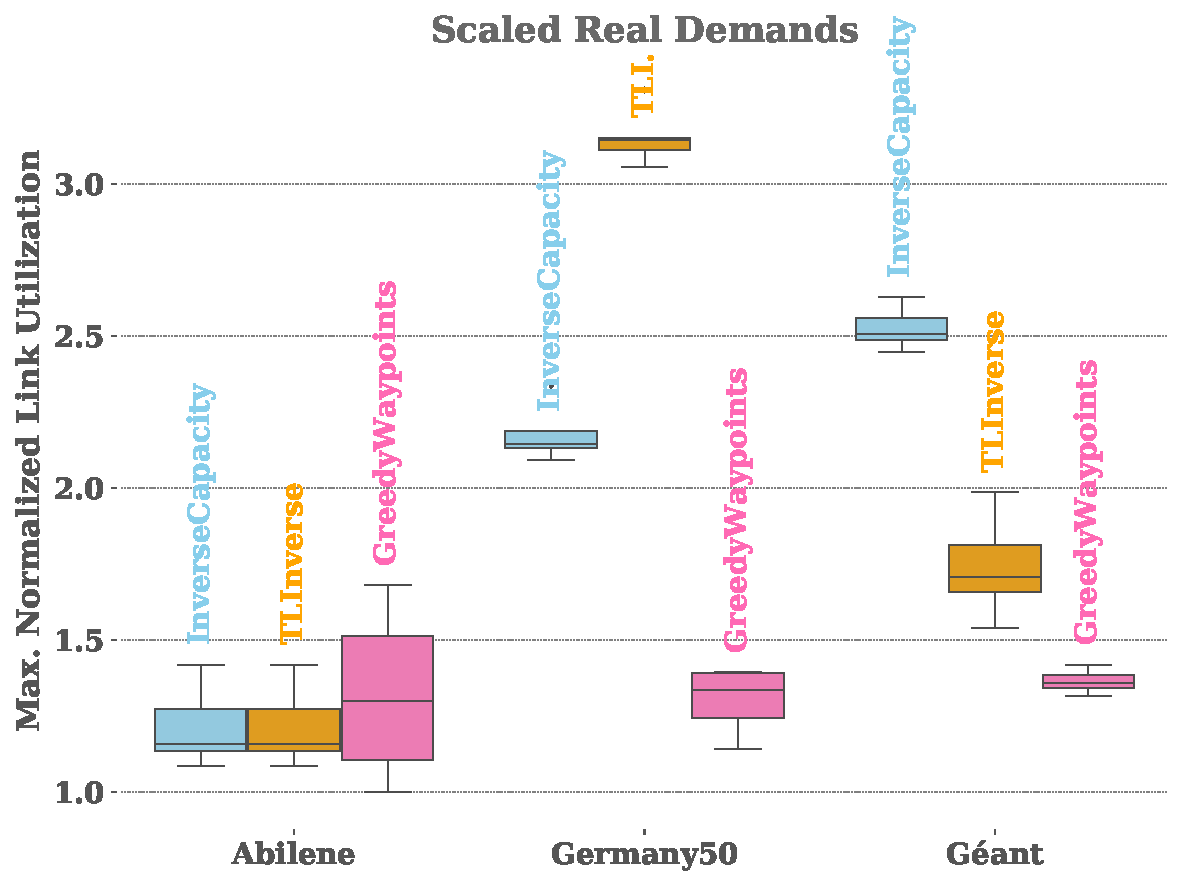
\includegraphics[width=.95\linewidth]{p1_alpha_07.pdf}
  \caption{Projekt 1 – TL\_Inverse, $\alpha=0{,}7$}
  \label{fig:p1-a07}
\end{figure}
\FloatBarrier
\noindent 
Über alle Topologien zeigt sich: Bei \(\alpha=0.3\) (vgl. Abb. 1) sind die Resultate praktisch
identisch zur \emph{inverse\_capacity}-Baseline—der Strafterm ist zu schwach, um Pfade spürbar zu verlagern.
Mit \(\alpha=0.5\) (vgl. Abb. 2) erzielt \textit{TL\_Inverse} einen guten Kompromiss: In \textbf{Géant} sinkt die MLU sichtbar, während in \textbf{Abilene} wegen geringer Pfadvielfalt kaum reagiert. Nur in \textbf{Germany50} kommt es zu einer erhöhten MLU, da durch die heterogene Struktur von \textbf{Germany50} neue Hotspots provoziert werden: Entlastete Kanten werden durch neu entstehende Engpässe auf Ausweichpfaden „ersetzt“, sodass die MLU nicht mehr konsistent fällt.
Erhöht man auf \(\alpha=0.7\)(vgl. Abb. 3), sehen wir ähnliche Ergebnisse wie für \(\alpha=0.5\).
 In Summe empfiehlt sich \(\alpha\approx0.5\) zu wählen, um effektive Ergebnisse für die verschiedenen Topologien zu erzielen. Der Einsatz von \textit{TL\_Inverse} sollte jedoch je nach Topologie gut überdacht sein, da er zu deutlich erhöhter MLU führen kann.

\subsection{Diskussion (TL\_Inverse)}
Die beobachteten Effekte von \textit{TL\_Inverse} lassen sich konsistent aus dem Wirkprinzip der Gewichtsaktualisierung in \eqref{eq:update} und der resultierenden Routenwahl erklären. Indem die Linkkosten proportional zur \emph{normierten} Auslastung $u_{ij}$ steigen, werden in der jeweils nächsten Iteration genau jene Kanten unattraktiver, die zuvor Engpässe gebildet haben. Der zentrale Stabilisator ist dabei die Skalierung \emph{relativ zur Basis} (\emph{vgl.} \eqref{eq:basew}): Da $w^{(k+1)}_{ij}$ stets aus $\mathrm{base\_w}_{ij}$ abgeleitet wird, kann die Metrik nicht ungebunden „davonlaufen“, sondern bleibt numerisch gebändigt. In Verbindung mit ECMP führt dies zu einer schrittweisen, aber kontrollierten Pfadverlagerung weg von Hotspots hin zu weniger belasteten Teilen der Topologie.

Gleichzeitig erklärt dieses Zusammenspiel die \(\alpha\)-Sensitivität: Für kleine Werte
(\(\alpha=0{,}3\)) ist die Modulation in \eqref{eq:update} so schwach, dass die induzierten Kostenunterschiede die Kürzeste-Pfade-Struktur praktisch nicht verändern; das Ergebnis fällt identisch zur \emph{inverse\_capacity}-Baseline aus. Bei moderaten Werten (\(\alpha=0{,}5\)) entsteht der intendierte Trade-off: Überlastete Links werden hinreichend penalisiert, ohne dass alternative Pfade übermäßig verteuert oder neue Ungleichgewichte erzeugt werden — insbesondere in gut vernetzten Graphen wie \textbf{Géant} senkt dies die MLU spürbar. Für hohe Werte (\(\alpha=0{,}7\)) kann die Anpassung hingegen \emph{übersteuern}: ECMP-Ties und diskrete Pfadwechsel führen dann zu nichtlinearen Sprüngen in der Lastverteilung, sodass Entlastung auf einer Kante durch neu entstehende Hotspots auf Ausweichrouten „bezahlt“ wird (\textbf{Germany50}). Das Verfahren bleibt zwar stabil (durch die Basis-Skalierung), optimiert die MLU aber nicht mehr monoton.

Die Topologie spielt dabei eine doppelte Rolle. In kleinen, relativ homogenen Netzen mit geringer Pfadvielfalt (\textbf{Abilene}) fehlen Alternativen, sodass selbst sinnvolle Gewichtsmodulationen kaum Wirkung entfalten. In mittelgroßen, gut vernetzten Netzen (\textbf{Géant}) existieren mehrere konkurrenzfähige, nur leicht längere Routen; hier entfaltet \textit{TL\_Inverse} den größten Nutzen. In größeren und heterogeneren Netzen (\textbf{Germany50}) steigen die Risiken von „Lastverschiebungen“: Kapazitätsunterschiede und längere alternative Wege können dazu führen, dass eine lokale Penalität global unerwünschte Nebenwirkungen erzeugt, wenn \(\alpha\) zu groß gewählt wird.

Als methodische Grenzen bleiben drei Punkte: Erstens ist der Strafterm in \eqref{eq:update} linear in $u_{ij}$; nichtlineare Varianten (z.\,B.\ saturierende oder stückweise lineare Formen) könnten Überreaktionen dämpfen, ohne den Reaktionsgrad bei moderater Auslastung zu verlieren. Zweitens optimiert \textit{TL\_Inverse} die MLU \emph{indirekt} über Gewichtssteuerung und ist damit empfindlich gegenüber ECMP-Tie-Breaking und diskreten Pfadwechseln; eine zusätzliche Regularisierung (z.\,B.\ Pfadlängen- oder Schwankungsterm) könnte hier Robustheit schaffen. Drittens betrachten wir ausschließlich die MLU als Zielgröße; in Praxis-Setups sind ergänzende Kriterien (Fairness, Pfadlänge, Latenzvariabilität) relevant und können Zielkonflikte mit der MLU aufdecken. Insgesamt legt die Analyse nahe, \(\alpha\) konservativ zu wählen (typisch um \(\alpha\approx0{,}5\)) und die Topologieeigenschaften (Pfaddiversität, Kapazitätsheterogenität)bei der Parametrisierung explizit zu berücksichtigen.

\subsection{Algorithmus \texorpdfstring{\textbf{demand\_first\_waypoints}}{demand_first_waypoints}}
Aufbauend auf der bekannten Demand-First-Waypoints-Heuristik verfolgen wir dasselbe Greedy-Prinzip,
lassen jedoch zwei gezielte Modifikationen einfließen. Erstens verwenden wir statt uniformer
Startkosten die kapazitätsbewussten Basisgewichte aus \eqref{eq:basew}, d.\,h.
\[
w^{(0)}_{ij}=\mathrm{base\_w}_{ij}=\max_{e\in E}c_e/c_{ij}
\] 
Damit bevorzugt die Kürzeste-Wege-Metrik
bereits vor der Waypoint-Suche Links mit höherem Headroom. Zweitens wird der ECMP-Split in seltenen
Randfällen numerisch robust gemacht (kein Divide-by-Zero, wohldefinierte Null-Anteile, falls temporär
keine gültigen Nachfolger vorliegen).

Der eigentliche Greedy-Schritt bleibt unverändert: Die Demands $(s,t,d)\in\mathcal D$ werden
absteigend nach Volumen verarbeitet, und es wird höchstens ein Waypoint $w\in V\setminus\{s,t\}$
zugelassen. Für jeden Kandidaten wird das Routing über $s\!\to\!w\!\to\!t$ (mit Dijkstra+ECMP unter
$w^{(0)}$) simuliert und die resultierende maximale Linkauslastung (MLU, vgl. Abschnitt~3.2) bewertet.
Wir wählen
\begin{equation}
w^\star \;=\; \arg\min_{w\in V\setminus\{s,t\}} \; \mathrm{MLU}\bigl(\text{Routen}(s{\to}w{\to}t; \, w^{(0)})\bigr)
\end{equation}
und übernehmen $w^\star$ nur, wenn die MLU \emph{strict} sinkt; anschließend wird die Lastkarte
aktualisiert und der nächste Demand bearbeitet. Die Kombination aus kapazitätsbewusster
Initialisierung und konservativem „ein Segment pro Demand“-Schema zielt darauf ab, Hotspots effektiv
zu entschärfen, ohne die Pfadstruktur aggressiv zu destabilisieren.

\subsection{Evaluationsdesign (DFW)}
Die Bewertung unserer Anpassung von \texttt{demand\_first\_waypoints} erfolgt auf denselben
Topologien wie zuvor (Abilene, Géant, Germany50) mit identischen, realistisch skalierten
Demand-Sätzen; Graph- und Kapazitätsmodell entsprechen Abschnitt~3.1. Als Referenz dient die
bekannte Demand-First-Waypoints-Baseline, gegen die wir ausschließlich die beiden Änderungen aus
Abschnitt~3.5 testen (inverse\_capacity-Startgewichte statt uniformer Kosten; robuster ECMP-Split).
Das Greedy-Schema bleibt ansonsten unverändert (ein Waypoint pro Demand, nur wenn die MLU sinkt).

Die Routenwahl geschieht deterministisch über Dijkstra+ECMP: Für jeden Demand werden nach der
Greedy-Entscheidung die kürzesten Wege relativ zu den \emph{fixen} Startgewichten verwendet; die
Lastberechnung und die Zielgröße \emph{MLU} folgen der Definition aus Abschnitt~3.2. Da das Verfahren
ohne iterative Gewichtsanpassung arbeitet, genügt ein einzelner Greedy-Durchlauf über alle Demands
(„demands first“). 

Wir berichten die Ergebnisse als Boxplots der MLU je Topologie (ohne Tabellen); die vertikale Achse
ist – analog zu den TL\_Inverse-Plots – bewusst gezoomt, um kleine, aber systematische Unterschiede
sichtbar zu machen.

\subsection{Ergebnisse (DFW)}
\begin{figure}[H]
  \centering
  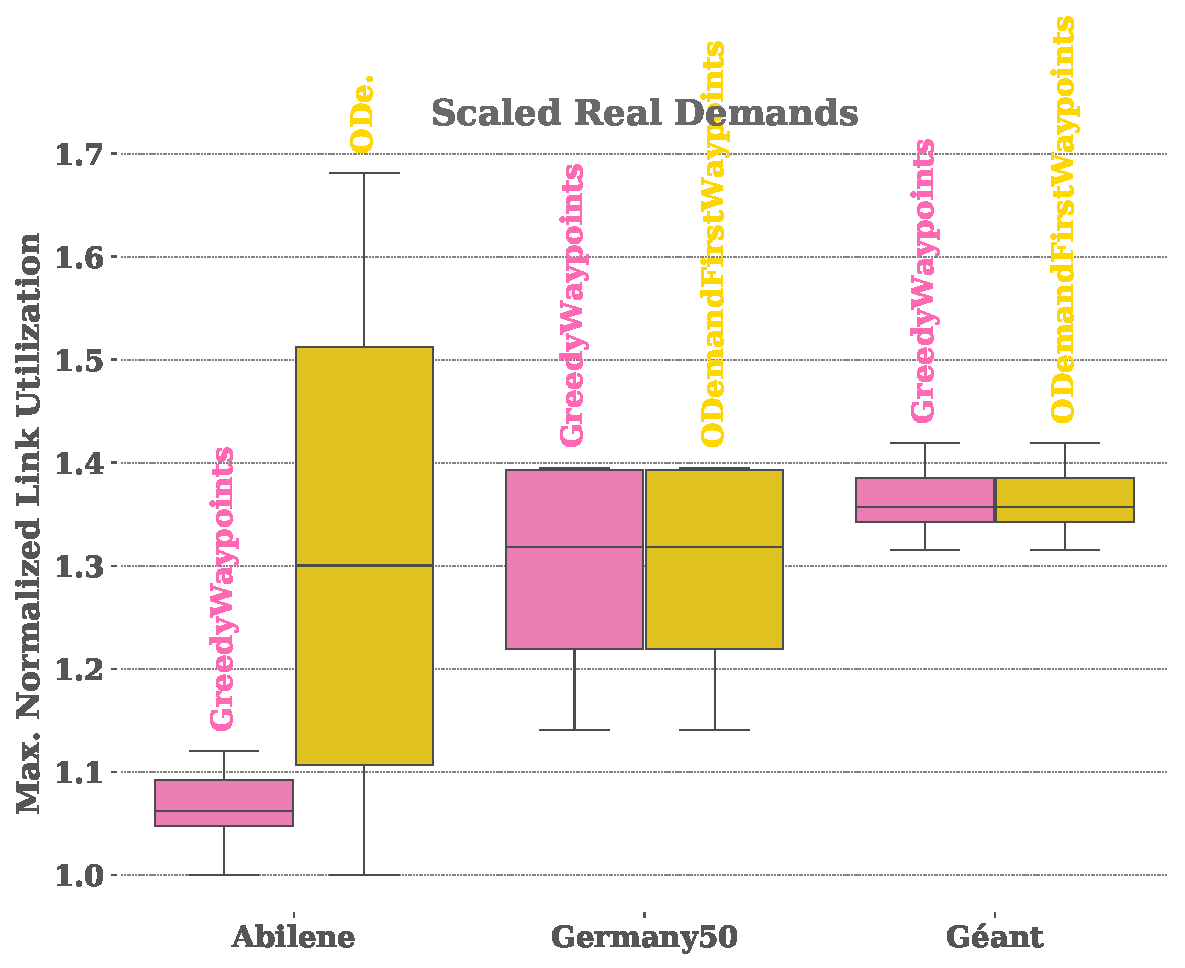
\includegraphics[width=.95\linewidth]{p1_dfw.pdf}
  \caption{Projekt 1 – DFW}
  \label{fig:p1-dfw}
\end{figure}
\FloatBarrier
\noindent
Über alle Topologien zeigt sich ein konsistentes Muster (vgl. Abb.~\ref{fig:p1-dfw}; die y-Achse ist gezoomt):
In \textbf{Abilene} fallen die Unterschiede gering aus, was der niedrigen Pfaddiversität entspricht.
In \textbf{Géant} profitiert unsere Variante von der kapazitätsbewussten Startmetrik und erzielt
häufig eine niedrigere MLU als die Baseline. Für \textbf{Germany50} hängt der Effekt stärker von der
Demandlage ab; Greedy-Entscheidungen können vereinzelt Last verlagern und damit neue Hotspots auf
Ausweichpfaden erzeugen, sodass die Vorteile nicht in allen Seeds konsistent sind. Insgesamt liefert
\emph{GreedyWaypoints} leichte Mediangewinne bei moderater Pfadvielfalt, während in sehr kleinen oder
sehr heterogenen Netzen die Robustheit der Verbesserungen begrenzt bleibt.

\subsection{Diskussion (DFW)}
Die Befunde lassen sich aus dem Zusammenspiel von kapazitätsbewusster Startmetrik und Greedy-Auswahl
(„ein Segment pro Demand“) erklären. Durch die Initialisierung $w^{(0)}_{ij}=\mathrm{base\_w}_{ij}$ aus
\eqref{eq:basew} verschiebt sich die Kürzeste-Wege-Metrik bereits vor der Waypoint-Suche in Richtung
kapazitätsstarker Links; der erste akzeptierte Waypoint wirkt daher häufig \emph{entlastend}, ohne schwache
Kanten unnötig zu beanspruchen. Diese Vorstrukturierung entfaltet ihren größten Nutzen dort, wo mehrere
konkurrenzfähige Alternativpfade existieren (Géant): Lokale Umlenkungen führen dann zu einer echten
Abflachung der Spitzenlast (MLU), ohne die Pfadlängen signifikant zu erhöhen.

Grenzen zeigen sich an beiden Enden des Spektrums: In Netzen mit geringer Pfadvielfalt (Abilene) fehlen
hinreichend gute Alternativen, sodass die Waypoint-Suche nur selten eine spürbare Verbesserung gegenüber
der Baseline erzielt. In größeren, heterogeneren Topologien (Germany50) kann die Greedy-Entscheidung
Last \emph{verlagern} statt sie zu neutralisieren, insbesondere wenn ECMP-Ties diskrete Sprünge in der
Routenwahl auslösen. Das erklärt die beobachtete Streuung: Einzelne Seeds profitieren deutlich, andere
erzeugen neue Hotspots auf Ausweichpfaden.

Methodisch ist die \emph{Single-Waypoint-Beschränkung} pro Demand der zentrale Trade-off zwischen
Einfachheit und Optimalkraft. Zwei natürliche Erweiterungen bieten sich an: (i) ein zweites Segment, das
nur bei weiterer MLU-Reduktion aktiviert wird (stufenweise Greedy-Suche), und (ii) eine hybride Kopplung
mit gewichtsbasierter Penalität (z.\,B. TL\_Inverse) zur Dämpfung von Überreaktionen bei ECMP-Ties.
Zudem ließe sich die Auswahl regelbasiert regularisieren (z.\,B. Mindestentlastungsschwelle, sanfte
Strafkosten für Pfadlängen-Inflation), um Varianz zu reduzieren, ohne den medianen Gewinn in
pfaddiversen Netzen zu verlieren.


\FloatBarrier
\section{Projekt 2\,\textemdash\,TE\_SR\_experiments}

\subsection{Zielsetzung \& Topologie (TL\_Inverse)}
Dieses Kapitel überträgt die in Projekt~1 untersuchten Ideen in eine nanonet-basierte Laufumgebung und betrachtet zwei Vergleichs­strecken: \emph{TL\_Inverse vs.\ New\_Weights} sowie \emph{DFW vs.\ Weights\_2}.
Für \textbf{TL\_Inverse vs.\ New\_Weights} nutzen wir einen gerichteten Graphen mit $|V|=6$ Knoten ($V=\{0,1,2,3,4,5\}$) und paarweise gerichteten Kanten. Die Kapazitäten sind heterogen: die innere Verbindung $0\leftrightarrow3$ ist mit $c_{03}=c_{30}=5$ der \emph{Bottleneck}, alle übrigen Links tragen $c_{ij}=10$ (Außenring als Ausweichstruktur). Die Demandmenge ist
\[
\mathcal{D}=\{(0,4,10),\ (0,5,5),\ (2,4,5),\ (1,5,5)\},
\]
wodurch mehrere Alternativrouten mit geringen Kostenunterschieden, aber potenziell unterschiedlicher Auslastung unter ECMP entstehen.

\subsection{Implementierung (TL\_Inverse)}
Die Pipeline ist reproduzierbar und identisch zur in Projekt~1 verwendeten Toolchain: Aus einer JSON-Beschreibung (Knoten, Kanten mit Kapazität, Demands) erzeugt \texttt{\nolinkurl{traffic_engineering_json2nanonet_v2_tl.py}} ein ausführbares \texttt{.topo.py}. Danach generiert \texttt{\nolinkurl{build.py}} daraus das \texttt{.topo.sh}, das Linux-Namespaces, Veth-Paare und Routingtabellen aufsetzt und die Messläufe startet. Die Routen werden in \texttt{\nolinkurl{dijkstra_computed()}} materialisiert (Dijkstra/ECMP, optional SR-Segmente). Pro Demand starten parallele \texttt{nuttcp}-Ströme (\texttt{NSTREAMS=32}) über \texttt{TIME=300\,s}; eine Startverzögerung von ca.\ 2\,min stellt die Initialisierung sicher. ECMP ist via Hash-Policy aktiv. Um vorzeitige Terminierungen auf leistungsschwacher VM zu vermeiden, wurde die Aufräumphase konservativ verzögert (z.\,B.\ \verb|sleep(self.TIME + 60)|), sodass \texttt{throughput.py -s} die Auswertung zuverlässig abschließt.

\emph{Abbildung der Verfahren:} \textbf{New\_Weights} setzt \emph{statisch} erhöhte Kosten auf dem Innenlink $0\leftrightarrow3$ (doppelte Linkkosten) und erzwingt per Segment Routing (SR) gewünschte Wege um den Engpass. \textbf{TL\_Inverse} startet mit gleichmäßigen Gewichten, führt eine vorgelagerte Lastschätzung aus und passt die Linkkosten proportional zur normierten Auslastung an (vgl.\ \eqref{eq:update}); die finalen Pfade werden als Multipath-Konfiguration mit Anteilsgewichten in die Topologie geschrieben. Alle übrigen Parameter (Topologie, Kapazitäten, Demands, Messdauer) sind zwischen den Varianten identisch.

\subsection{Baselines \& Metrik (TL\_Inverse)}
Verglichen werden \textbf{New\_Weights} (deterministische SR-Policy mit manuell verteuertem Bottleneck) und \textbf{TL\_Inverse} (datengetriebene, lastadaptive Gewichtssteuerung). Die Routenwahl erfolgt in beiden Fällen über Dijkstra mit ECMP. Zielgröße ist die \emph{maximale Linkauslastung (MLU)}; Definition und Lastberechnung entsprechen Abschnitt~3.2. Weitere Kriterien (Fairness, Pfadlänge, Jitter) optimieren wir hier bewusst nicht, um den Einfluss der Routenwahl auf Hotspot-Bildung isoliert zu betrachten.

\subsection{Ergebnisse \& Einordnung (TL\_Inverse)}
\begin{figure}[H]
  \centering
  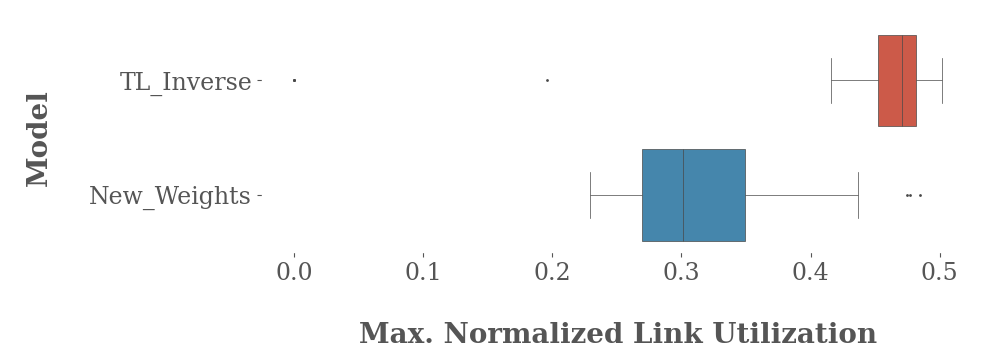
\includegraphics[width=.9\linewidth]{TL_New_Weights.png}
  \caption{Projekt 2 — TL\_Inverse.}
  \label{fig:p2-tl}
\end{figure}
\noindent
Die Ergebnisse in \autoref{fig:p2-tl} zeigen einen \emph{leicht} niedrigeren Median und eine geringere Streuung für \textit{New\_Weights} gegenüber \textit{TL\_Inverse}. Die gezoomte y-Achse verdeutlicht, dass die absoluten Differenzen klein sind; beide Verfahren liegen in einem engen MLU-Band. Der Vorteil der Baseline erklärt sich durch die Kombination aus \emph{statisch verteuertem Innenlink} und \emph{SR-Policy}, die die Umgehung des Bottlenecks deterministisch erzwingt. \textit{TL\_Inverse} verteilt Last adaptiv, kann bei geringer Pfaddiversität jedoch neue Belastungsschwerpunkte auf Ausweichpfaden erzeugen und den Median nicht weiter senken. Insgesamt deuten die Resultate darauf hin, dass manuell getunte SR-Policies in kleinen, gut kontrollierbaren Topologien robuste leichte Vorteile liefern, während adaptive Verfahren ihren Mehrwert eher in dynamischeren oder variablen Situationen entfalten.

\subsection{Zielsetzung \& Topologie (DFW vs.\ Weights\_2)}
Für die zweite Vergleichsstrecke konstruieren wir eine kompakte, SR-fähige Topologie mit \textbf{fünf Knoten}
($0$–$4$) und zwei Kapazitätsklassen: \textbf{80\,Mbit/s} auf den Außenkanten ($0\!\leftrightarrow\!1$,
$0\!\leftrightarrow\!3$, $1\!\leftrightarrow\!4$, $3\!\leftrightarrow\!4$) sowie \textbf{40\,Mbit/s} auf
allen Kanten über \emph{Knoten 2} ($0\!\leftrightarrow\!2$, $1\!\leftrightarrow\!2$, $2\!\leftrightarrow\!3$,
$2\!\leftrightarrow\!4$). Die Demands sind symmetrisch und je \textbf{10\,Mbit/s}: $0\!\to\!4$, $4\!\to\!0$,
$1\!\to\!3$, $3\!\to\!1$. Knoten 2 bildet damit einen Innen-Hub mit geringerer Kapazität; über den Außenring
stehen belastbare Alternativpfade bereit.

\subsection{Implementierung (DFW vs.\ Weights\_2)}
Die Artefakte werden analog erzeugt (JSON $\to$ \texttt{.topo.py} $\to$ \texttt{.topo.sh}); Mess- und
Systemparameter entsprechen Strecke A (\texttt{TIME=300\,s}, \texttt{NSTREAMS=32}, Startoffset $\approx$ 2\,min,
ECMP aktiv; konservative Terminierung zur Vermeidung abgebrochener Läufe). In \textbf{Weights\_2} sind die
\emph{Linkkosten uniform} (z.\,B.\ 1000), SR-Waypoints werden \emph{nicht} gesetzt; die Routen entstehen
rein durch Dijkstra/ECMP. In \textbf{DFW} werden die \emph{Linkkosten kapazitätsbewusst} gesetzt (z.\,B.\ 2000
auf 40\,Mbit/s, 1000 auf 80\,Mbit/s); zusätzlich erzwingen wir pro Demand \emph{einen SR-Waypoint}
(z.\,B.\ $0\!\to\!4$ via 1, $4\!\to\!0$ via 3, $1\!\to\!3$ via 4, $3\!\to\!1$ via 0) mittels
\texttt{encap seg6 ... segs \{w\}}. Damit spiegelt Strecke B den methodischen Unterschied der Idee wider:
kapazitätsbewusste Vorstrukturierung plus wohldosiertes, deterministisches Segment im Vergleich zu einer
uniformen Weights-Baseline.

\subsection{Baselines \& Metrik (DFW vs.\ Weights\_2)}
Verglichen werden \textbf{DFW} (GreedyWaypoints, kapazitätsbewusste Kosten, fester Single-Waypoint pro Demand)
und \textbf{Weights\_2} (uniforme Kosten, keine Waypoints). Als Zielgröße verwenden wir die MLU aus Abschnitt~3.2;
alle übrigen Parameter (Demands, Seeds, Messdauer) sind zwischen den Varianten identisch. Ergebnisse berichten wir
als Boxplots, um Median und Streuung gegenüberzustellen.

\subsection{Ergebnisse \& Einordnung (DFW vs.\ Weights\_2)}
\begin{figure}[H]
  \centering
  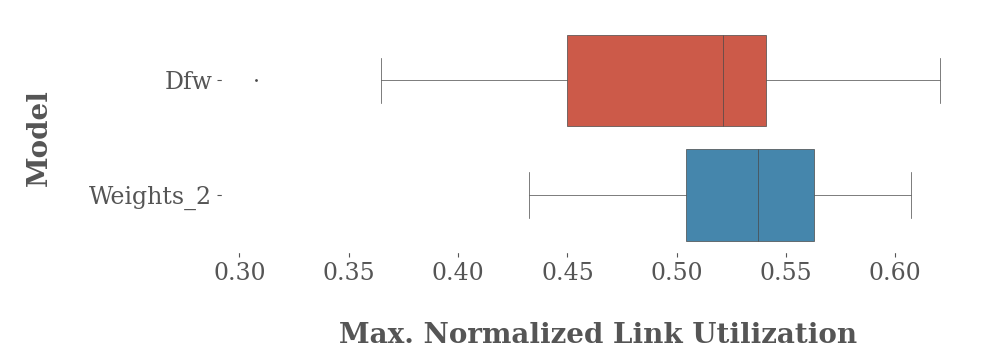
\includegraphics[width=.9\linewidth]{Dfw_weights_2.png}
  \caption{Projekt 2 — DFW.}
  \label{fig:p2-dfw}
\end{figure}
\noindent
Die Median-MLU beider Varianten liegt nahe beieinander; \emph{DFW} ist im Median leicht im Vorteil, zeigt jedoch
eine größere Streuung. \emph{Weights\_2} liefert eine engere Box (stabiler), liegt dafür minimal höher. Die
absoluten Unterschiede sind klein (gezoomte Achse). Interpretatorisch passt das Bild zur Konstruktion: Die
Kombination aus kapazitätsbewusster Metrik und erzwungenen SR-Segmenten umgeht den Innen-Bottleneck zuverlässig,
erhöht aber die Varianz abhängig von ECMP-Aufteilung und Segmentwahl. Die uniforme Baseline ist robuster, jedoch
nicht immer median-optimal. Zusammen mit Strecke A ergibt sich damit ein konsistentes Gesamtbild: Auf kleinen,
gezielt designten Topologien können deterministische SR-Policies einen stabilen Vorteil liefern, während adaptive
und/oder kapazitätsbewusste Strategien leichte Mediangewinne erzielen, deren Robustheit mit der Pfaddiversität
und der konkreten Demandlage variiert.


\FloatBarrier
\section{Limitierungen \& Validität}
Die Aussagekraft der Ergebnisse wird durch mehrere Validitätsaspekte begrenzt, die wir im Folgenden transparent machen und, wo möglich, mit getroffenen Gegenmaßnahmen verknüpfen.

\paragraph{Interne Validität.}
Die Implementierungen orientieren sich strikt an den in Kapitel~3 eingeführten Definitionen: \emph{TL\_Inverse} aktualisiert Gewichte relativ zur Basis (\eqref{eq:basew}) gemäß (\ref{eq:update}); die Auswertung erfolgt nach fixierten $K$ Iterationen. Für \emph{DFW} (unsere Anpassung von \texttt{demand\_first\_waypoints}) verwenden wir kapazitätsbewusste Startgewichte ($w^{(0)}_{ij}=\mathrm{base\_w}_{ij}$) sowie einen robusten ECMP-Split, der Divide-by-Zero vermeidet. Gleichwohl verbleiben Risiken: Wir haben keine \emph{formale Konvergenz-/Laufzeitanalyse} für \emph{TL\_Inverse} durchgeführt (nur $K{=}3$ in den Experimenten), und bei \emph{DFW} erzwingt die Single-Waypoint-Beschränkung eine Heuristik, die lokale Optima begünstigen kann. In \textit{Projekt~2} traten auf der genutzten VM vorzeitige Terminierungen auf; zur Absicherung wurde die Aufräumphase konservativ verzögert (\texttt{sleep(self.TIME + 60)}), damit alle Läufe vollständig in \texttt{throughput.py -s} einfließen. Diese Maßnahme reduziert Messabbrüche, eliminiert jedoch nicht mögliche \emph{System-Noise} (Scheduling, CPU-Steal) der VM. Sämtliche Läufe nutzen identische Parameter (z.\,B.\ \texttt{NSTREAMS=32}, \texttt{TIME=300\,s}, einheitliche ECMP-Hash-Policy), um Implementationsartefakte von algorithmischen Effekten zu trennen.

\paragraph{Konstruktvalidität.}
Wir fokussieren bewusst die \emph{maximale Linkauslastung (MLU)} als Zielgröße. Diese konservative Kenngröße erfasst Hotspots unmittelbar, blendet jedoch andere für den Betrieb relevante Aspekte (Pfadlänge, Latenz/Jitter, Fairness) aus. Insbesondere bei \emph{TL\_Inverse} kann eine MLU-Verbesserung mit leichten Pfadlängen-Zunahmen einhergehen; bei \emph{DFW} kann die lokale Umlenkung Pfade selektiv verlängern. Auch die ECMP-Semantik (gleichmäßige Aufteilung bei gleichen Kosten) ist Teil des Konstrukts: Tie-Breaking und diskrete Pfadwechsel können Lastsprünge verursachen, die sich in der MLU widerspiegeln, ohne dass die Gesamtnetzqualität zwingend schlechter wäre. Unsere qualitative Interpretation macht diese Grenzen transparent, ersetzt aber keine Multi-Ziel-Optimierung.

\paragraph{Externe Validität.}
Die drei WAN-Topologien (Abilene, Géant, Germany50) decken ein Spektrum aus Größe, Konnektivität und Heterogenität ab, bleiben aber Repräsentanten; die Übertragbarkeit auf größere ISP-Backbones, Traffic-Diurnalität oder hochvariable Demand-Matrizen ist nicht automatisch gegeben. Die in \textit{Projekt~2} entworfenen Topologien sind \emph{absichtlich klein} und SR-fähig, um Mechanismen isoliert sichtbar zu machen; daraus folgen klare, aber kontextgebundene Aussagen. Zudem setzt \emph{DFW} in \textit{Projekt~2} feste Waypoints je Demand ein—eine starke Annahme, die in produktiven Netzen durch Policy-/SR-Constraints, Tailoring und Operationspraxis limitiert sein kann.

\paragraph{Statistische Schlussfolgerungsvalidität.}
Wir berichten Ergebnisse primär über Boxplots (Median/Streuung) und verzichten auf formale Signifikanztests oder umfangreiche Seed-Studien. Die y-Achsen wurden \emph{gezoomt}, um kleine, aber systematische Unterschiede sichtbar zu machen; dadurch wirken Abstände optisch größer als in absoluten Werten. Insbesondere in \textit{Projekt~2} sind die Differenzen zwischen Baseline und Variante \emph{klein}; unsere Einordnung bleibt daher \emph{qualitativ} und betont Trends statt harter Schwellen.

\paragraph{Maßnahmen zur Absicherung.}
Wir halten die Vergleichsbedingungen zwischen Baselines und Varianten konstant (Topologie, Kapazitäten, Demands, \texttt{NSTREAMS}, Messdauer, ECMP-Policy). Für \emph{TL\_Inverse} variieren wir $\alpha\in\{0.3,0.5,0.7\}$, um Sensitivität sichtbar zu machen; für \emph{DFW} beschränken wir Änderungen strikt auf Startmetrik und ECMP-Robustheit. Die erfolgreiche \emph{Replikation} fremder Ergebnisse in beiden Projekten stützt die korrekte Umsetzung der Toolchains und erhöht die Nachvollziehbarkeit. Alle verwendeten Artefakte (JSON/\texttt{.topo.py}/\texttt{.topo.sh}, Plots) sind versioniert abgelegt und im Quellenanhang referenziert.

\paragraph{Implikationen.}
Die Resultate sind \emph{valide im Sinne des gewählten Konstrukts} (MLU unter Dijkstra+ECMP/SR) und der betrachteten Topologien. Für breitere Generalisierungen empfehlen sich (i) zusätzliche Zielfunktionen (Pfadlänge, Fairness, Jitter), (ii) Sensitivitätsstudien über Demands/Seeds und (iii) größere, realitätsnahe Topologien. Methodisch bieten sich als Erweiterungen nichtlineare Strafterme bzw.\ adaptive $\alpha$ (für \emph{TL\_Inverse}) sowie Multi-Segment-Greedy oder Hybride (Waypoint $+$ Gewichtsmodulation) für \emph{DFW} an, um Varianz zu dämpfen, ohne Median-Vorteile zu verlieren.


\FloatBarrier
\section{Fazit}
\textbf{Fazit.}
Die beiden betrachteten Ansätze adressieren die Reduktion der maximalen Linkauslastung (MLU) komplementär:
\emph{TL\_Inverse} erweitert die inverse\_capacity-Metrik um eine auslastungsadaptive Komponente und zeigt in
mittelgroßen, gut vernetzten Netzen (Géant) konsistente Vorteile, während in sehr kleinen, homogenen Topologien
(Abilene) die Pfaddiversität zu gering ist, um spürbare Effekte zu entfalten. In heterogeneren Netzen (Germany50)
ist die Wahl von $\alpha$ maßgeblich; moderat gewählte Werte (ca.\ $\alpha\!\approx\!0{,}5$) balancieren Entlastung
und Stabilität am zuverlässigsten. Im nanonet-Setting (Projekt~2) liegt \emph{New\_Weights} leicht vorn,
da die Kombination aus manuell verteuertem Bottleneck und deterministischer SR-Policy die Umgehung des Engpasses
erzwingt und auf der bewusst kleinen Topologie sehr gut zur Demandlage passt; die absoluten Unterschiede bleiben
gleichwohl klein. Unsere angepasste Waypoint-Heuristik \emph{DFW} profitiert von der
kapazitätsbewussten Startmetrik: In pfaddiversen Szenarien liefert sie leichte Mediangewinne (Projekt~1/Géant),
während sie in Projekt~2 gegenüber der uniformen Weights-Baseline einen minimalen Medianvorteil bei höherer
Streuung zeigt. Insgesamt ergibt sich ein konsistentes Bild: deterministische, manuell getunte SR-Policies
liefern in kleinen, gut kontrollierbaren Topologien robuste, leicht bessere Mediane; adaptive bzw.\ kapazitäts­
bewusste Strategien reagieren datengetrieben und können in geeigneten Topologien MLU-Vorteile erzielen, allerdings
mit stärkerer Varianz. Die erfolgreichen Replikationen stützen die korrekte Umsetzung und erhöhen die Nachvollziehbarkeit
der Befunde.

\clearpage
\section{Replikation (fremde Ergebnisse)}

\subsection{Projekt 1\,\textemdash\,TE\_SR\_WAN\_simulation}
\begin{figure}[H]
  \centering
  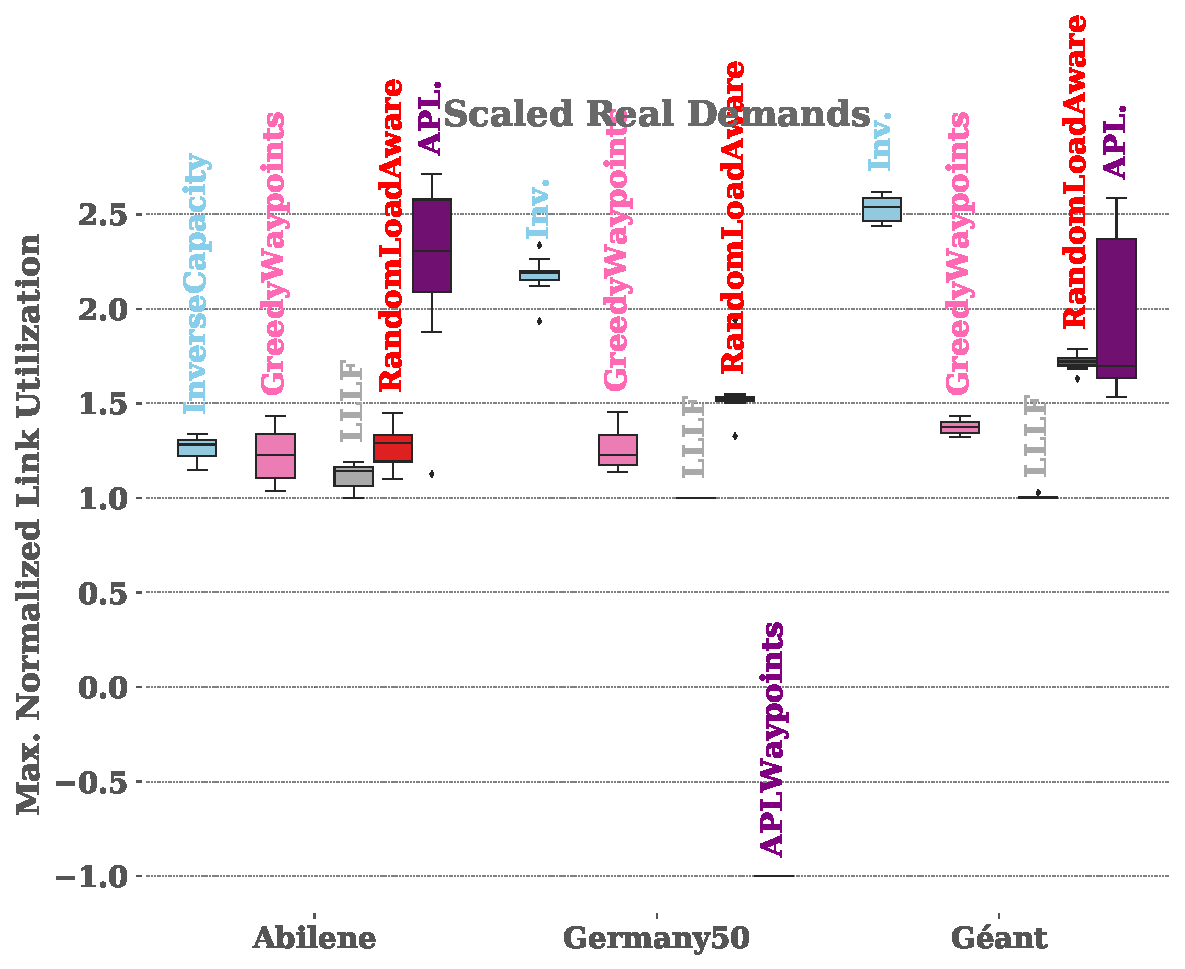
\includegraphics[width=.95\linewidth]{p1_replication.pdf}
  \caption{Projekt~1 — Replikation: MLU über Abilene, Géant und Germany50 (fremde Ergebnisse, repliziert).}
  \label{fig:p1-repl}
\end{figure}
\noindent
Zur Überprüfung der Nachvollziehbarkeit haben wir die Resultate einer anderen Gruppe für
\textbf{Abilene}, \textbf{Géant} und \textbf{Germany50} repliziert (vgl.\ Abb.~\ref{fig:p1-repl}).
Nach kleineren Startschwierigkeiten (Umgebung/Pfade, initiale Skriptaufrufe) liefen die
Messungen vollständig durch und konnten ausgewertet werden. (vgl. Abb. 7)

\subsection{Projekt 2\,\textemdash\,TE\_SR\_experiments (Gruppe 3)}
\begin{figure}[H]
  \centering
  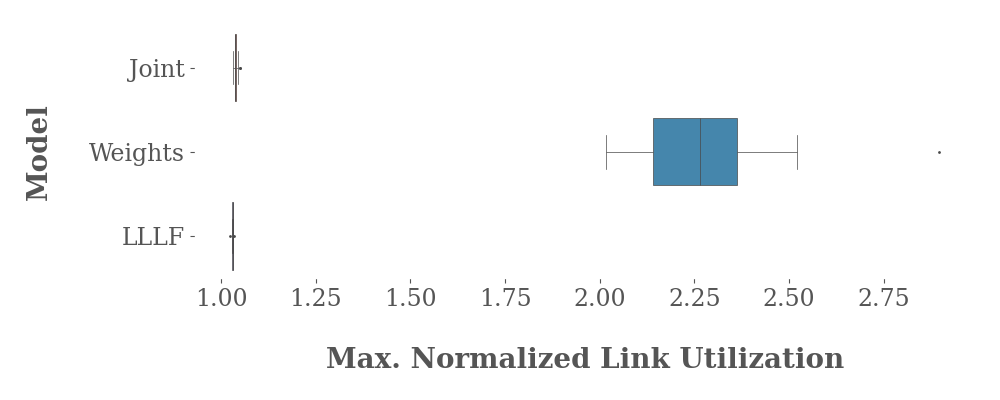
\includegraphics[width=.9\linewidth]{results.png}
  \caption{Projekt~2 — Replikation: Ergebnisse Gruppe~3 (Boxplot-Übersicht).}
  \label{fig:p2-repl-results}
\end{figure}
\begin{figure}[H]
  \centering
  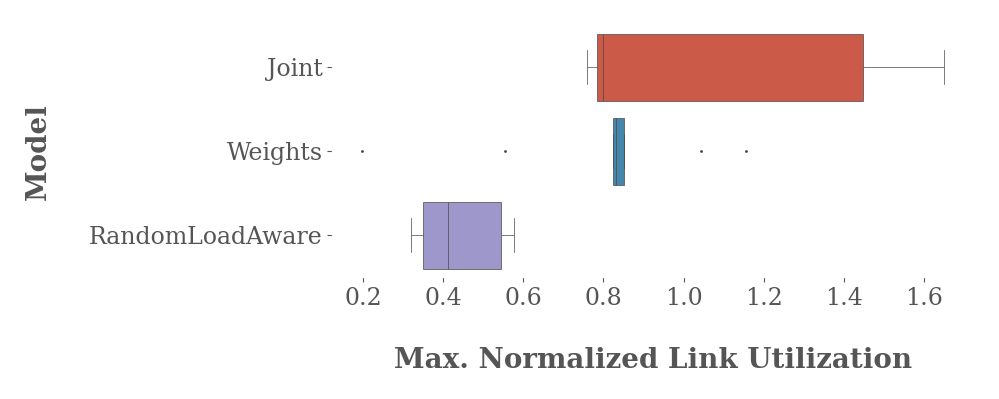
\includegraphics[width=.9\linewidth]{GraphRLA.png}
  \caption{Projekt~2 — Replikation: Graph RLA (Darstellung der Resultate).}
  \label{fig:p2-repl-graph}
\end{figure}
\begin{figure}[H]
  \centering
  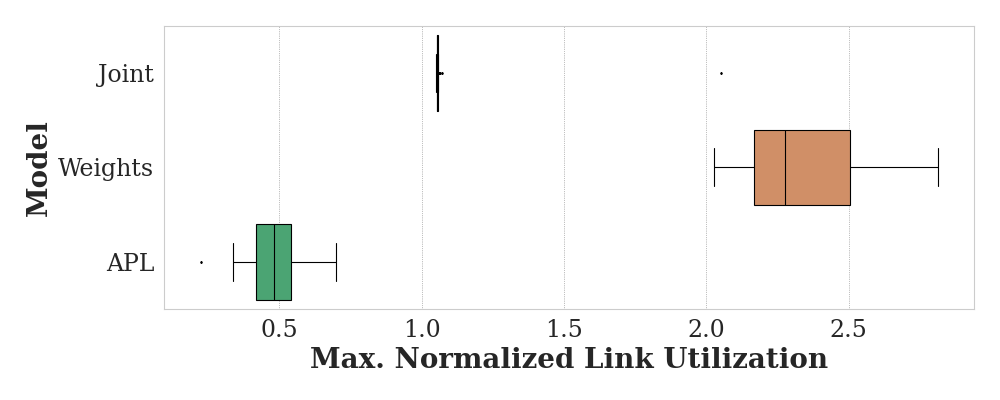
\includegraphics[width=.9\linewidth]{result_02.png}
  \caption{Projekt~2 — Replikation: Result\_02 (Boxplot-Detail).}
  \label{fig:p2-repl-detail}
\end{figure}
\FloatBarrier
\noindent
Die Replikation der Ergebnisse von \textbf{Gruppe~3} im \textit{TE\_SR\_experiments}-Setup konnte
\emph{weitgehend problemlos} über \texttt{nanonet\_batch} durchgeführt werden. Auf der genutzten
VM traten jedoch vereinzelt vorzeitige Terminierungen auf; zur Absicherung wurde die Aufräumphase
konservativ verzögert (\verb|sleep(self.TIME + 60)| in \texttt{nanonet\_batch}), sodass
\texttt{throughput.py -s} vollständige Messergebnisse verarbeiten konnte. Die replizierten
Boxplots und Graphdarstellungen (Abb.~\ref{fig:p2-repl-results}–\ref{fig:p2-repl-detail})
reproduzieren die qualitativen Muster der Originalaussagen.
Insgesamt stützen die Replikationen die korrekte Umsetzung der
Toolchain und erhöhen die Nachvollziehbarkeit der im Report gezogenen Schlüsse.


\clearpage
\onecolumn
\section*{Literatur / Quellen}
\textbf{Basis/Frameworks}\\
\begin{itemize}
  \item \textbf{TE\_SR\_WAN\_simulation:} \url{https://github.com/tfenz/TE_SR_WAN_simulation}
  \item \textbf{TE\_SR\_experiments\_2021:} \url{https://github.com/nikolaussuess/TE_SR_experiments_2021}
  \item \textbf{Nanonet:} \url{https://github.com/nikolaussuess/nanonet}
\end{itemize}
\medskip
\textbf{Eigene Repositories (Ergebnisse/Implementierung)}\\
\begin{itemize}
  \item \textbf{Projekt 1:} \url{https://github.com/Fisch96/Results_fachprojekt_group_4}
  \item \textbf{Projekt 2:} \url{https://github.com/Fisch96/TE_SR_experiments_2021-Gruppe4}
\end{itemize}
\medskip
\textbf{Replizierte Gruppen/Repos}\\
\begin{itemize}
  \item \textbf{Gruppe 3 Projekt 1:} \url{https://github.com/Makeandbreak09/TE_SR_WAN_simulation}
  \item \textbf{Gruppe 3 Projekt 2:} \url{https://github.com/Makeandbreak09/TE_SR_experiments_2021}
\end{itemize}

\end{document}
